

%% Basierend auf einer TeXnicCenter-Vorlage von Mark Müller
%%%%%%%%%%%%%%%%%%%%%%%%%%%%%%%%%%%%%%%%%%%%%%%%%%%%%%%%%%%%%%%%%%%%%%%

% Wählen Sie die Optionen aus, indem Sie % vor der Option entfernen  
% Dokumentation des KOMA-Script-Packets: scrguide

%%%%%%%%%%%%%%%%%%%%%%%%%%%%%%%%%%%%%%%%%%%%%%%%%%%%%%%%%%%%%%%%%%%%%%%
%% Optionen zum Layout des Artikels                                  %%
%%%%%%%%%%%%%%%%%%%%%%%%%%%%%%%%%%%%%%%%%%%%%%%%%%%%%%%%%%%%%%%%%%%%%%%
\documentclass[%
%a5paper,							% alle weiteren Papierformat einstellbar
%landscape,						% Querformat
12pt,								% Schriftgröße (12pt, 11pt (Standard))
%BCOR1cm,							% Bindekorrektur, bspw. 1 cm
%DIVcalc,							% führt die Satzspiegelberechnung neu aus
%											  s. scrguide 2.4
%twoside,							% Doppelseiten
%twocolumn,						% zweispaltiger Satz
%halfparskip*,				% Absatzformatierung s. scrguide 3.1
%headsepline,					% Trennline zum Seitenkopf	
%footsepline,					% Trennline zum Seitenfuß
titlepage,						% Titelei auf eigener Seite
%normalheadings,			% Überschriften etwas kleiner (smallheadings)
%idxtotoc,						% Index im Inhaltsverzeichnis
%liststotoc,					% Abb.- und Tab.verzeichnis im Inhalt
%bibtotoc,						% Literaturverzeichnis im Inhalt
%abstracton,					% Überschrift über der Zusammenfassung an	
%leqno,   						% Nummerierung von Gleichungen links
%fleqn,								% Ausgabe von Gleichungen linksbündig
%draft								% überlangen Zeilen in Ausgabe gekennzeichnet
bibliography=totoc
]
{scrartcl}

\usepackage{geometry}
\geometry{a4paper, left=45mm, right=20mm, top=30mm, bottom=30mm}
% http://www.macuser.de/forum/f19/latex-zeilenabstand-aendern-189206/
\usepackage{setspace}

% Hurenkinder und Schusterjungen verhindern
\clubpenalty10000
\widowpenalty10000
\displaywidowpenalty=10000

\usepackage[flushmargin,hang,ragged]{footmisc}

%\pagestyle{empty}		% keine Kopf und Fußzeile (k. Seitenzahl)
%\pagestyle{headings}	% lebender Kolumnentitel  


%% Deutsche Anpassungen %%%%%%%%%%%%%%%%%%%%%%%%%%%%%%%%%%%%%
\usepackage[ngerman]{babel}
\usepackage[T1]{fontenc}
\usepackage[ansinew]{inputenc}
\usepackage{graphicx}

\usepackage{lmodern} %Type1-Schriftart für nicht-englische Texte
\usepackage{fancyhdr}

%\usepackage{cite}
%\renewcommand{\citeleft}{}
%\renewcommand{\citeright}{}

%% Packages für Grafiken & Abbildungen %%%%%%%%%%%%%%%%%%%%%%
\usepackage{graphicx} %%Zum Laden von Grafiken
%\usepackage{subfig} %%Teilabbildungen in einer Abbildung
%\usepackage{pst-all} %%PSTricks - nicht verwendbar mit pdfLaTeX

%% Beachten Sie:
%% Die Einbindung einer Grafik erfolgt mit \includegraphics{Dateiname}
%% bzw. über den Dialog im Einfügen-Menü.
%% 
%% Im Modus "LaTeX => PDF" können Sie u.a. folgende Grafikformate verwenden:
%%   .jpg  .png  .pdf  .mps
%% 
%% In den Modi "LaTeX => DVI", "LaTeX => PS" und "LaTeX => PS => PDF"
%% können Sie u.a. folgende Grafikformate verwenden:
%%   .eps  .ps  .bmp  .pict  .pntg

%% Bibliographiestil %%%%%%%%%%%%%%%%%%%%%%%%%%%%%%%%%%%%%%%%%%%%%%%%%%
\usepackage[style=authoryear,backend=bibtex8]{biblatex}
\usepackage[babel,german=quotes]{csquotes}
%\addbibresource{Literatur.bib}
\bibliography{./Literatur}

\begin{document}
\parskip=1em
\parindent=0cm
\pagestyle{empty} %%Keine Kopf-/Fusszeilen auf den ersten Seiten.


%%%%%%%%%%%%%%%%%%%%%%%%%%%%%%%%%%%%%%%%%%%%%%%%%%%%%%%%%%%%%%%%%%%%%%%
%% Ihr Artikel                                                       %%
%%%%%%%%%%%%%%%%%%%%%%%%%%%%%%%%%%%%%%%%%%%%%%%%%%%%%%%%%%%%%%%%%%%%%%%

%% eigene Titelseitengestaltung %%%%%%%%%%%%%%%%%%%%%%%%%%%%%%%%%%%%%%%    
%\begin{titlepage}
%Einsetzen der TXC Vorlage "Deckblatt" möglich
%description: Deckblatt in Deutsch
%% Basierend auf einer TeXnicCenter-Vorlage von Tino Weinkauf.
%%%%%%%%%%%%%%%%%%%%%%%%%%%%%%%%%%%%%%%%%%%%%%%%%%%%%%%%%%%%%%

%%%%%%%%%%%%%%%%%%%%%%%%%%%%%%%%%%%%%%%%%%%%%%%%%%%%%%%%%%%%%
%% Deckblatt
%%%%%%%%%%%%%%%%%%%%%%%%%%%%%%%%%%%%%%%%%%%%%%%%%%%%%%%%%%%%%
%%
%% ACHTUNG: Sie ben�tigen ein Hauptdokument, um diese Datei
%%          benutzen zu k�nnen. Verwenden Sie im Hauptdokument
%%          den Befehl "\input{dateiname}", um diese
%%          Datei einzubinden.
%%

\begin{titlepage}
\vspace{5cm}
Stefan Waidele \hfill{} Matthias Vongerichten\\
Immatrikulationsnr. 1028171 \hfill{} Immatrikulationsnr. 1038859\\
Ensisheimer Stra�e 2 \hfill{} Hauptstra�e 96\\
79395 Neuenburg am Rhein \hfill{} 76877 Offenbach a. d. Queich\\
Stefan.Waidele@AKAD.de \hfill{} Matthias.Vongerichten@AKAD.de

\vfill

\begin{tabbing}
Modul INT02 --- \=Einf�hrung in die Internetprogrammierung\\ 
                \>Assignment  
\end{tabbing}
\LARGE
\textsc{Erstellung einer Website \\f�r ein fiktives Busunternehmen}\\

\vfill

\normalsize
Betreuer: Andr� Langbein

\today %%Datum der Abgabe - am besten selbst reinschreiben.

\vfill

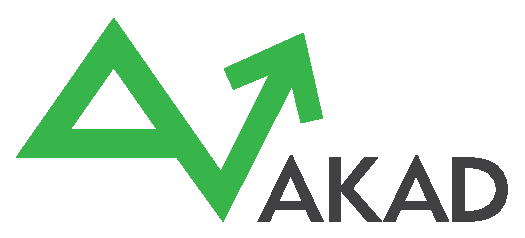
\includegraphics[width=3cm]{AKAD-Logo}

AKAD Hochschule Stuttgart

\end{titlepage}
%\end{titlepage}

%% Erzeugung von Verzeichnissen %%%%%%%%%%%%%%%%%%%%%%%%%%%%%%%%%%%%%%%
\setcounter{tocdepth}{2}
\tableofcontents			% Inhaltsverzeichnis
%\listoftables				% Tabellenverzeichnis
\listoffigures				% Abbildungsverzeichnis
\clearpage


%% Der Text %%%%%%%%%%%%%%%%%%%%%%%%%%%%%%%%%%%%%%%%%%%%%%%%%%%%%%%%%%%
\pagestyle{headings}
\begin{onehalfspacing}
\section{Einleitung}
\subsection{Ziel der Arbeit}

Ziel dieser Arbeit ist die Erstellung einer Website f�r ein fiktives Busunternehmen ohne Zuhilfenahme von speziellen WYSIWYG Website-Editoren oder CMS--Systemen.

F�r die Website sind jeweils ein redaktionelles, ein Gestaltungs-- und ein Navigationskonzept zu erstellen. Von jedem Teammitglied ist eine Einzelseite des Internetauftritts zu erstellen.

Das Ziel dieser Arbeit ergibt sich direkt aus der Aufgabenstellung im Rahmen des AKAD--Studienmoduls "`INT02 -- Einf�hrung in die Internetprogrammierung"'

\subsection{Vorgehensweise}

\begin{itemize}
	\item Im Kapitel "`Anforderungsanalyse"' werden die Grundlagen f�r die zu erarbeitenden Konzepte kurz beschrieben.
				Es handelt sich hierbei aufgrund der rein fiktiven Aufgabenstellung eher die Beschreibung der von den Autoren 
				getroffenen Annahmen als um eine tats�chliche Analyse.
	\item In den folgenden Kapiteln wird die Website bez�glich den Inhalten, der Navigation und des Designs geplant.
	\item Jeder der beiden Autoren realisiert eine konkrete Seite und beschreibt die hierzu eingesetzten Methoden.
\end{itemize}


\subsection{Abgrenzung}

Lediglich zwei Seiten des Internetauftritts werden im Rahmen dieser Arbeit im Detail betrachtet.
Die �brigen werden lediglich in den zu erarbeitenden Konzepten besprochen, ohne jedoch tats�chlich erstellt zu werden.

Ebenfalls wird nicht die gesamte Planung der Internetpr�senz\footnote{vgl. \cite{kyas}, S274} in dieser Arbeit besprochen. Des Weiteren sollten die hier erarbeiteten Konzepte im Einklang mit den Vorgaben der Marketingstrategie stehen. Da hier lediglich ein fiktives Unternehmen betrachtet wird, besteht eine solche Strategie nicht.

Die komplette Realisierung einer echten Unternehmenswebsite w�rde hier noch weitere Analyse-- Planungs-- und Arbeitsschritte erfordern.

Es wird kein Social--Media--Konzept erstellt, da dies den Rahmen der Arbeit �berschreiten w�rde. Allerdings wird die Einbindung von Web 2.0 Komponenten im Rahmen des Redaktionellen Konzepts betrachtet.
\section{Anforderungsanalyse}

\subsection{Ziele der Website}

Die Unternehmenswebsite f�gt sich in die gro�e Bandbreite der Werbema�nahmen eines Unternehmens ein.
Daher muss diese sich auch nach den Grunds�tzen der Werbung und des Marketings richten.

Die allgemeinen Ziele der Website sind die Gewinnung neuer Kunden sowie die Erh�hung des Bekantheitsgrades des Unternhemens.

F�r diese Arbeit gehen wir von folgendenden Vorgaben\footnote{\cite{kloss}, S. 183ff} aus:

\begin{itemize}
	\item \textbf{Zielgruppe:}\\
	Das Unternehmen betrachtet Alleinreisende und Paare im Alter zwischen 40 und 65 Jahren als die Hauptzielgruppe f�r die angebotenen St�dtereisen. Au�erdem sollen Vereine und Reisegruppen gemischten Alters angesprochen werden. 
	Altersunabh�ngig ist die Zielgruppe haupts�chlich den Sinus-Charakteristiken "`B�rgerliche Mitte"', "`Traditionelle"' oder "`Konservativ--etablierte"' zuzuordnen\footnote{\cite{sinus}}.
	
	\item \textbf{Phase der Buchungsentscheidung:}\\
	Die Website soll dem Kunden zu jedem Zeitpunkt des Entscheidungsvorgangs\footnote{vgl. \cite{freyer}, S105} etwas bieten k�nnen. Es ist jedoch besonders auf die Informations-- und Handlungsphase zu achten, da hier der Einfluss des Unternehmens am direktesten ist.
\end{itemize}

\subsection{Funktionale Anforderungen}

Folgende Funktionen sollten dem Besucher der Seite angeboten werden:

\begin{itemize}
	\item Vermitteln von Informationen �ber das Unternehmen
	\item Darstellung der Reiseziele und deren Details
	\item Buchung von Reisen
	\item Kontaktaufnahme mit dem Unternehmen
\end{itemize}

\subsection{Nicht-funktionale Anforderungen}

Folgenden nicht--funktionalen bzw.qualitativen Kriterien soll die Website entsprechen:

\begin{itemize}
	\item Abgestimmtes Erscheinungsbild
	\item Kurze Ladezeiten
	\item Einfaches Zurechtfinden
	\item Einfache Kontaktaufnahme
	\item Wenig Administrationsaufwand
	\item Mehrsprachigkeit (Deutsch, Englisch)
\end{itemize}

Dar�ber hinaus sind die Dialoggrunds�tze f�r interaktive Systeme gem�� ISO 9241-110 zu beachten\footnote{\cite{bhofmann}}:

\begin{itemize}
	\item Aufgabenangemessenheit
	\item Selbstbeschreibungsf�higkeit
	\item Erwartungskonformit�t
	\item Fehlertoleranz
	\item Steuerbarkeit
	\item Individualisierbarkeit
	\item Lernf�rderlichkeit
\end{itemize}

\subsection{Technische Voraussetzungen}

Zum Betreiben der Website wird ein Webspace mit mindestens 50MB Speicherplatz, vorzugsweise unlimitiertem Traffic, FTP-Zugang, und der M�glichkeit der mod\_rewrite--Aktivierung ben�tigt. Au�erdem muss der verwendete Webserver PHP interpretieren k�nnen. Eine Datenbank ist nicht erforderlich. F�r das Bearbeiten der Seiteninhalte gen�gt ein Text--Editor.
Zur besseren Auffindbarkeit der Website wird eine Top-Level-Domain empfohlen. Diese kann dem Webspace oft einfach zugebucht werden.
\section{Redaktionelles Konzept}

\textsc{Mathias Vongerichten bzw. Stefan Waidele}

\subsection{Startseite}

Nicht ausdr�cklich gefordert, sollte aber dabei sein.

\subsection{Kurzdarstellung des Unternehmens}

...

\subsection{Reiseziele}

In L�nder�bersicht und Reisedetails gegliedert. Inkl. Termine und Preise.

\subsection{Informationen �ber �bernachtungsm�glichkeiten}

...

\subsection{Informationen zu den Bussen}

...

\subsection{Preise}

Inkl. Termine?

\subsection{Buchungsm�glichkeiten}

\subsubsection{Telefon}
\subsubsection{Schriftlich: Brief, Fax, E-Mail}
Evt. Zitat aus meinem ANS03-Assignment: "`E-Mail = Brief"'

\subsubsection{HTML--Formular}

...

\subsubsection{Internet Booking Engine -- IBE}

...

\subsection{Social--Media Einbindung}

Kein eigenes Social--Media--Konzept, da nur Website gefordert

Twitter-Feed auf Homepage oder als eigene Seite (gefiltert nach Hashtag) --- Pro und Contra

Kommentarfunktion bei einzelnen Reisen

Einbindung von Bewertungsportalen (Customer--Alliance Demo-Siegel?)

\subsection{Noch Konzept...}

...

\section{Navigationskonzept - MV}

\textsc{Mathias Vongerichten bzw. Stefan Waidele}

\subsection{Techniche Umsetzung einheitlicher Navigation}

Eine Zentrale PHP-Datei liest in die einheitliche Struktur die Details der Seite ein. Parameter�bergabe in der URL mit Apache Mod-Rewrite (wg. SEO).

\subsection{Seitenhierarchie}

Nicht zu tief.

\subsection{Men�struktur}

...

\subsection{Breadcrumb Navigation}

Jedenfalls mit deutscher �berschrift.

\subsection{Related Pages}

Je Reiseziel ein Abschnitt mit interessanten externen Links

\subsection{Suchmaschinenoptimierung}

META-Tags, Verweis auf redaktionelles Konzept f�r Content-Strategie etc.

\subsection{Noch Konzept...}

...

\section{Designkonzept}

\textsc{Matthias Vongerichten bzw. Stefan Waidele}

\subsection{Einheitliche Darstellung durch CSS}

...

\subsection{Gliederung der Seiten durch DIVs}

\subsubsection{Beurteilung TABLE}

Layout mit HTML-Tabellen ist B�SE!

\subsubsection{Beurteilung FRAME}

Layout mit HTML-Frames ist SCHLECHT!

\subsubsection{Beurteilung CSS-DIV}

Layout mit DIVs per CSS ist GUT!

(Sematisches Markup, Reihenfolge weniger relevant, erm�glicht Liquid/Responsive Layout, ...

\subsection{Farbkonzept}

...

\subsection{Richtlinien f�r Grafiken}

ALT-Tags

\subsection{Responsive Layout}

Mit Breakpoints f�r 1920px (HD), 960px (Klasisch Desktop), 800px (Beamer, Tablet), 480px (Smartphone)

Zwischenstufen Liquid.

\subsection{Special Effects}

Animationen (Dezent, evt. "`umdrehen"' bei Men�-MouseOver, Dezentes leuchten der Buchungs-Telefonnummer,...)

\subsection{Browserkompatibilit�t}

How far back in time do we want to travell?

\subsection{Noch Konzept...}

...

%%\section{Beispielseite: Startseite - MV}

\textsc{Mathias Vongerichten bzw. Stefan Waidele}

\subsection{�berschrift}

Erl�uterungen zur redaktionellen, gestalterischen und technischen Umsetzung.


%%\section{Beispielseite: L�nder�bersicht}

\textsc{Mathias Vongerichten bzw. Stefan Waidele}

\subsection{�berschrift}

Erl�uterungen zur redaktionellen, gestalterischen und technischen Umsetzung.

Die von uns erstellten Seiten sollten hier im Detail mit Screenshots und Alternativen vorgestellt werden. Seiten, die wir nicht erstellen k�nnen wir in einem Kapitel zusammenfassen.
\section{Beispielseite: Kontakt}

\textsc{Matthias Vongerichten}

\begin{figure}[h]
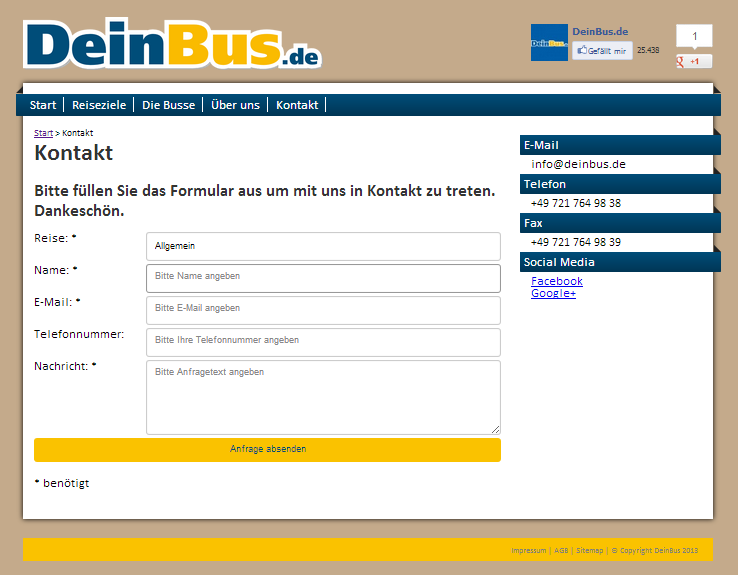
\includegraphics[width=\hsize]{scr_kontakt}
\caption{Screenshot: Kontaktformular}
\label{scr:kontakt}
\end{figure}

Die Seite "`Kontakt"' besteht zum gr��ten Teil aus einem Kontaktformular und den alternativen Kontaktm�glichkeiten in der Sidebar. 


\subsection{Validierung per HTML5}
Das Kontaktformular verwendet das �bliche HTML--Tag \code{Form} sowie einige HTML5--Funktionen. Erkennbar ist dies z.B. an dem Attribut \code{required}, welches dem Browser signalisiert, dass dieses Formularelement ausgef�llt werden muss. Versucht der Benutzer das Formular abzuschicken erh�lt er einen Hinweis �ber das leere Element und wird aufgefordert es auszuf�llen --- vorausgesetzt der Browser ist HTML5--kompatibel. Das Formular wird wie in Abbildung ~\ref{abb:formular} gezeigt durch eine �bliche, und hier auch semantisch gerechtfertigte, Tabelle strukturiert (HTML--Table Tag).

\begin{figure}[h]
\begin{minted}[bgcolor=bg]{html}
<tr>
   <td>Name: *</td>
   <td>
      <input id          ="name"  
             placeholder ="Bitte Name angeben" 
             type        ="text" 
             tabindex    ="1" 
             required 
             autofocus
      >
   </td>
</tr>
\end{minted}
\caption{Quellcode: Formular (HTML)}
\label{abb:formular}
\end{figure}

\subsection{Validierung per JavaScript}

F�r den Fall einer fehlenden HTML5--Unterst�tzung wurde eine Fallback--L�sung mittels JavaScript implementiert. Die Pr�fung auf eine HTML5--Unterst�tzung wurde wie wie in Abbildung ~\ref{abb:required} gezeigt umgesetzt und wird bei jedem Abschicken des Formulars durchgef�hrt.

\begin{figure}[h]
\begin{minted}[bgcolor=bg]{javascript}
var inputs = document.createElement('input');
var supports = {};
supports.required  = 'required' in inputs;

if(!supports.required) {
   /*...siehe unten...*/
}
\end{minted}
\caption{Quellcode: HTML5 oder JavaScript--Fallback (JavaScript)}
\label{abb:required}
\end{figure}

\subsection{Eingabefokus auf dem fehlerhaften Element}

Trifft die Pr�fung zu und HTML5 wird nicht unterst�tzt wird jedes auszuf�llende Formularelement auf dessen Inhalt gepr�ft. Bei einem Fehler wird die Formular�bermittlung abgebrochen und der Fokus auf das betroffene Element gesetzt (Siehe Abbildung ~\ref{abb:fokus}).

\begin{figure}[h]
\begin{minted}[bgcolor=bg]{javascript}
name = document.getElementById("name").value;
/*...*/
if (name == "")
{
   document.getElementById("name").select();
   document.getElementById("name").focus();
   return false;
}
\end{minted}
\caption{Quellcode: Fokussteuerung bei fehlerhaften Eingaben (JavaScript)}
\label{abb:fokus}
\end{figure}

\subsection{�berpr�fung der E--Mail Adresse}

Da HTML5 auch die Plausibilit�t von E--Mail Adressen pr�ft wurde auch dies im Fallback mit einer entsprechenden Abfrage ber�cksichtigt (Siehe Abbildung ~\ref{abb:test}). 

\begin{figure}[h]
\begin{minted}[bgcolor=bg]{javascript}
if (!checkEmail(email))
{
   alert('E-Mail ist ung�ltig.');
   return false;
}
\end{minted}
\caption{Quellcode: Abfrage: E--Mail Adresse g�ltig? (JavaScript)}
\label{abb:test}
\end{figure}

In der darin aufgerufenen Funktion wurde mithilfe des regul�ren Ausdrucks in Abbildung ~\ref{abb:regex} auf eine g�ltige E--Mail Adresse getestet

\begin{figure}[h]
\begin{minted}[bgcolor=bg]{javascript}
function checkEmail(inputvalue) {
   var pattern = /^([a-zA-Z0-9_\.\-])\
                  +\@(([a-zA-Z0-9\-])+\.)\
                  +([a-zA-Z0-9]{2,4})+$/;
   return pattern.test(inputvalue);
}
\end{minted}
\caption{Quellcode: Regul�rer Ausdruck: E--Mail Adresse (JavaScript)}
\label{abb:regex}
\end{figure}
\clearpage

%%\section{Beispielseite: Informationen zur Unterkunft - MV}

\textsc{Mathias Vongerichten bzw. Stefan Waidele}

\subsection{�berschrift}

Erl�uterungen zur redaktionellen, gestalterischen und technischen Umsetzung.


%%\section{Beispielseite: Informationen �ber die Busse}

\textsc{Mathias Vongerichten bzw. Stefan Waidele}

\subsection{�berschrift}

Erl�uterungen zur redaktionellen, gestalterischen und technischen Umsetzung.


%%\section{Beispielseite: Unternehmensportrait}

\textsc{Mathias Vongerichten bzw. Stefan Waidele}

\subsection{�berschrift}

Erl�uterungen zur redaktionellen, gestalterischen und technischen Umsetzung.


%%\section{Beispielseite: Impressum}

\textsc{Matthias Vongerichten bzw. Stefan Waidele}

\subsection{�berschrift}

Erl�uterungen zur redaktionellen, gestalterischen und technischen Umsetzung.


\section{Fazit}

Das redaktionelle Konzept beschreibt die vorgesehenen Inhalte je Seite in Kurzform. Au�erdem wird hierbei auch eine Richtlinie zur Aktualisierungsh�ufigkeit je Seite vorgegeben (unterst�tzt SEO). Somit wird erreicht, dass der redaktionelle Verantwortliche eine kompakte Anleitung zur Pflege der Website erh�lt.

Beim Navigationskonzept wurden die wichtigsten Navigationselemente beachtet. Hervorzuheben sind hier die "`Breadcrumb"'-Navigation und die Implementierung von mod\_rewrite (Abbildung ~\ref{abb:htaccess}, Seite ~\pageref{abb:htaccess}).

Durch die Formatierung der Website mithilfe von CSS kan der Redakteur sich im Wesentlichen auf die Inhalte bzw. auf die in einem zu erstellenden Handbuchs korrekte Auszeichnung mit relativ einfachen HTML--Tags konzentrieren, und nicht auf die Gestaltung der Website.

\begin{figure}[h]
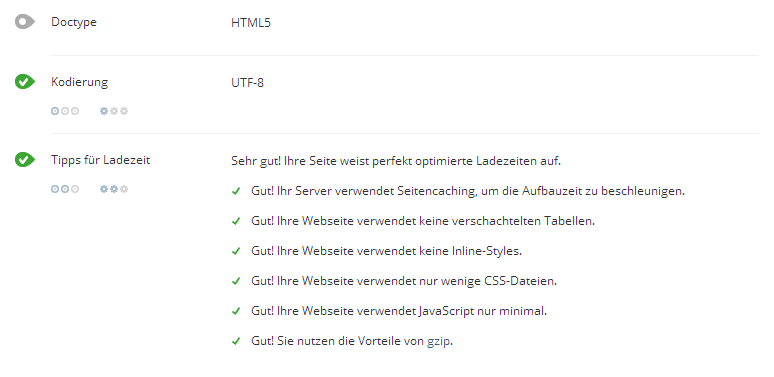
\includegraphics[width=\hsize]{scr_woorank_performance.png}
\caption{Screenshot: Performance}
\label{scr:performance}
\end{figure}

Die Website erf�llt die gestellten Anforderungen vollst�ndig. So bescheinigt, wie die Abbildungen~\ref{scr:performance} und~\ref{scr:mobile} zeigen, das SEO--Analyse--Tool \code{woorank.com}, dass z.B. nicht-funktionalen Anforderungen wie die Performance der Site sehr gut erf�llt werden. Durch den Einsatz von Media--Queries wird eine gro�e Bandbreite von Ger�ten unterst�tzt. Optimierungspotential ergibt sich hier noch durch eine m�gliche auf die Bildschirmgr��e abgestimmte Auslieferung der Grafiken. Dies w�rde aber den in der Aufgabenstellung vorgegebenen Rahmen an notwendigem Know--How f�r die Pflege der Website bzw. den Verzicht auf externe Hilfsmittel sprengen. 

\begin{figure}[h]
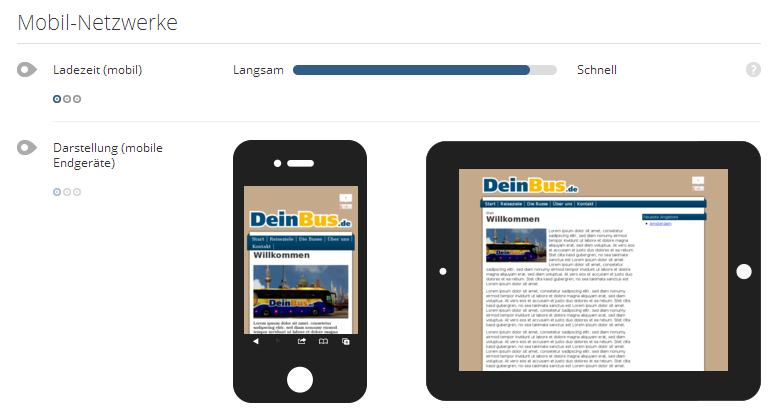
\includegraphics[width=\hsize]{scr_woorank_mobile_performance.png}
\caption{Screenshot: Mobile Ger�te}
\label{scr:mobile}
\end{figure}

Somit liegt ein n�chster m�glicher Schritt nahe, n�mlich die Verwendung eines Content-Management-Systems (CMS). Dies erm�glicht das einfache Bearbeiten der Seiteninhalte mithilfe eines WYSIWYG-Editors (keine Code-Kenntnisse notwendig) und das Aufrechterhalten eines konsistenten Designs. 

Die Navigation kann auf mehrere Ebenen und Elemente verteilt werden und aktualisiert sich selbst�ndig. Der Administrationsaufwand wird somit stark reduziert und trotzdem f�llt es erstaunlich leicht die Funktionen der Website durch vorgefertigte Module zu erweitern. So ist es ebenfalls m�glich einen Weblog zu betreiben welcher mit Facebook und anderen Social-Media-Diensten integriert werden kann. 

Urspr�nglich als Weblog-System zu gro�er Bekanntheit gelangt, kann Wordpress heute als einfaches und komfortables CMS genannt werden. F�r komplexere Anwendungsf�lle eignet sich Drupal oder Typo3.

Abschlie�end l�sst sich feststellen, dass der Betrieb einer Website heute mit den kostenlos angebotenen und doch professionellen Systemen deutlich besser und einfacher m�glich ist, als mit selbst erstelltem Code. Trotzdem werden auch hier ein redaktionelles-- und ein Navigationskonzept ben�tigt. Beim Design w�re abzuw�gen, ob man eine fertige, zur Firma passende Designvorlage\footnote{je nach System gibt es eine gro�e Auswahl von Designvorlagen, bzw. Themes oder auch Templates} �bernimmt, oder ob man sich von einem Dienstleister ein perfekt passendes Design f�r das gew�hlte CMS erstellen l�sst.



\end{onehalfspacing}

%% Bibliographie unter Verwendung von dinnat %%%%%%%%%%%%%%%%%%%%%%%%%%
%\setbibpreamble{Präambel}		% Text vor dem Verzeichnis
%\bibliographystyle{natdin}
%\bibliographystyle{plaindin}
%\bibliography{Literatur}	% Sie benötigen eine *.bib-Datei

%% Bibliographie unter Verwendung von BibLaTeX %%%%%%%%%%%%%%%%%%%%%%%%%%
\clearpage
\flushleft
\setlength{\bibitemsep}{1em}
\printbibliography

\clearpage

\pagestyle{empty} 
\thispagestyle{empty}

\textsc{\Large Eidesstattliche Erkl"arung}
\vspace*{4cm}

Ich versichere, dass ich das beiliegende Assignment selbstst"andig verfasst, keine anderen als die angegebenen Quellen und Hilfsmittel benutzt sowie alle w"ortlich oder sinngem"a"s "ubernommenen Stellen in der Arbeit gekennzeichnet habe. 
\vspace{3cm}

\begin{tabbing}
Wherever, \today \hspace{1em} \=\rule[-0.8ex]{6.5cm}{0.75pt}\\
                \>(Matthias Vongerichten) 
\end{tabbing}
\vspace{3cm}

\begin{tabbing}
Neuenburg am Rhein, \today \hspace{1em} \=\rule[-0.8ex]{6.5cm}{0.75pt}\\
                \>(Stefan Waidele) 
\end{tabbing}


\end{document}
